\section{Intercambios entre entidades} \label{sec:intercambio}
Para mostrar un ejemplo de intercambio entre entidades he realizado tres pruebas:
\begin{enumerate}
 \item El cliente pide un recurso al Service Provider y no está autenticado.
 \item El cliente pide un recurso al Service Provider y está autenticado.
 \item El cliente pide un recurso al Service Provider 2 y está autenticado.
\end{enumerate}

Las pruebas se han realizado de manera consecutiva. La correspondencia de las direcciones IP es la siguiente:
\begin{center}
\begin{tabular}{| l | c |}
	\hline
	\textbf{Entidad} & \textbf{IP} \\ \hline \hline 
	Cliente & 192.168.1.12 \\ \hline
	Service Provider & 192.168.1.140 \\ \hline
	Service Provider 2 & 192.168.1.134 \\ \hline
	Identity Provider & 192.168.1.135 \\ \hline
\end{tabular}
\end{center}

\subsubsection*{Primer intercambio}
En la figura \ref{fig:int1} se ve el intercambio número uno. Este consiste en la petición de un recurso al Service Provider sin que el cliente esté autenticado.

\begin{figure}[h!]
\centering
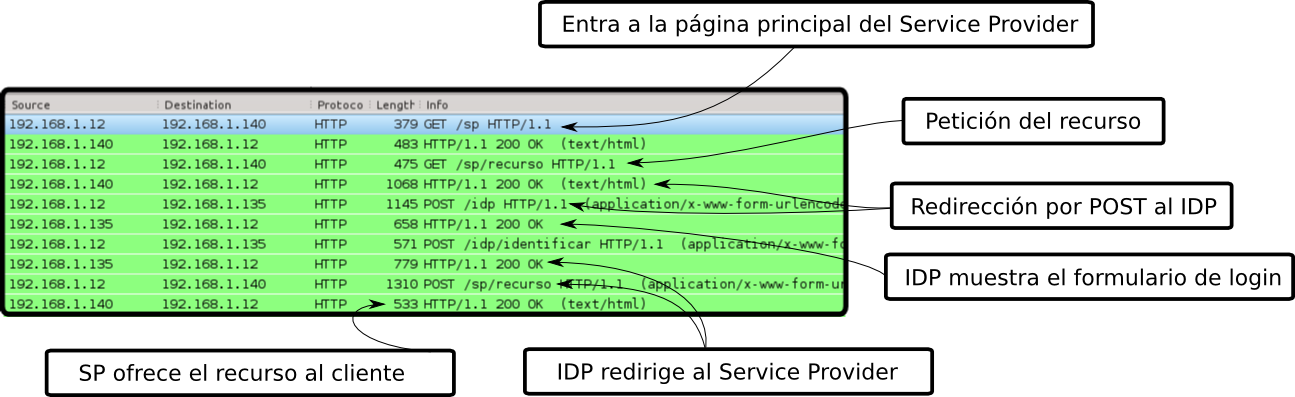
\includegraphics[width=\textwidth]{img/intercambio1-comentado}
\caption{Petición inicial del recurso.}
\label{fig:int1}
\end{figure}

A continuciación describo con detalle el intercambio:
\begin{enumerate}
 \item El cliente entra en la página principal del Service Provider, http://sp.seg.um/sp.
 \item El cliente solicita un recurso protegido.
 \item El Service Provider ve que la sesión del cliente no está autenticada, por lo que emite una página que le redirige al Identity Provider (por el método POST) junto con un Authentication Request.
 \item El cliente reenvía la petición al Identity Provider.
 \item El Identity Provider responde al cliente mostrándole el formulario de autenticación, donde el cliente introduce su usuario y contraseña.
 \item El Identity Provider autentica correctamente al usuario y le redirige al recurso solicitado del Service Provider enviando un Response.
 \item El Service Provider recibe el Response y ve que el usuario fue autenticado correctamente. A partir de ahora, el cliente tiene acceso a los recursos.
 \item El Service Provider ofrece el recurso al cliente.
\end{enumerate}

\subsubsection*{Segundo intercambio}
El segundo intercambio (figura \ref{fig:int2}) consiste en una petición al Service Provider estando ya autenticado el cliente:

\begin{figure}[h!]
\centering
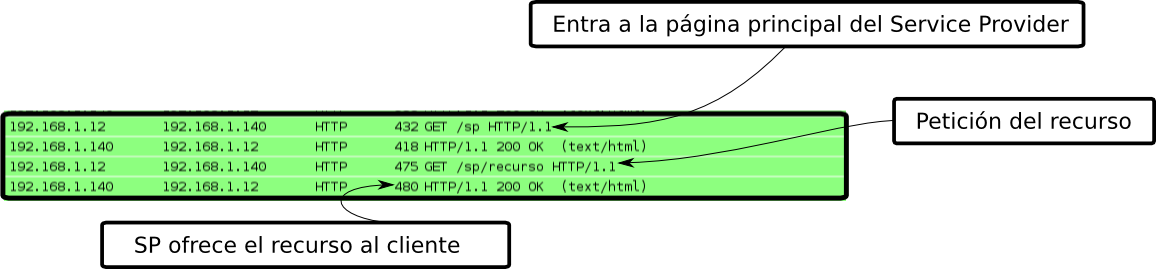
\includegraphics[width=\textwidth]{img/intercambio2-comentado}
\caption{Petición del recurso ya autenticado.}
\label{fig:int2}
\end{figure}

\begin{enumerate}
 \item El cliente entra en la página principal.
 \item El cliente solicita el recurso.
 \item El Service Provider recibe los datos de la sesión del cliente y ve que ya está autenticado en el Identity Provider.
 \item El Service Provider ofrece el recurso directamente al cliente.
\end{enumerate}

\subsubsection*{Tercer intercambio}
El tercer intercambio (figura \ref{fig:int3}) muestra al cliente accediendo a un recurso en otro Service Provider (llamado Service Provider 2).

\begin{figure}[h!]
\centering
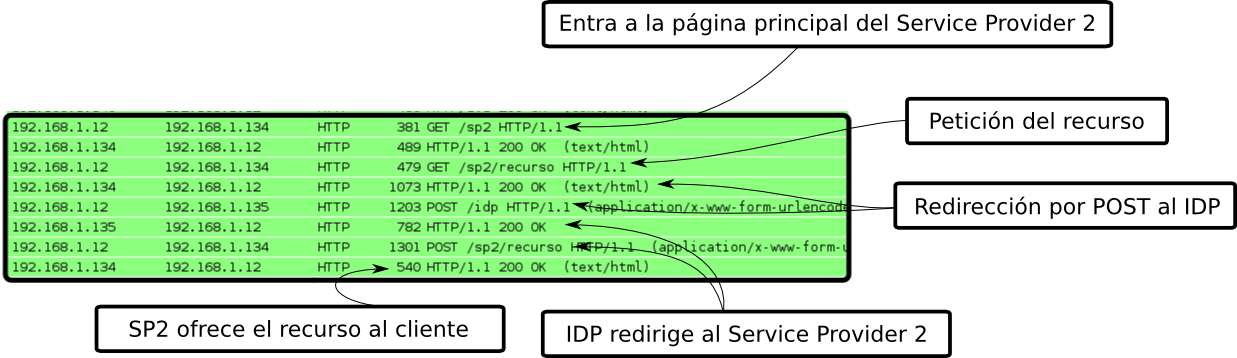
\includegraphics[width=\textwidth]{img/intercambio3-comentado}
\caption{Petición de un recurso en otro Service Provider ya autenticado.}
\label{fig:int3}
\end{figure}

\begin{enumerate}
 \item El cliente, tras acceder a la página principal (http://sp2.seg.um/sp2) solicita acceso al recurso protegido.
 \item El cliente es redirigido por POST al Identity Provider para autenticación, ya que éste no está autenticado en el sistema propio.
 \item El Identity Provider identifica al cliente automáticamente y le considera autenticado.
 \item Reenvía un Response al Service Provider 2.
 \item Service Provider 2 devuelve el recurso.
\end{enumerate}

\begin{figure}[h!]
\centering
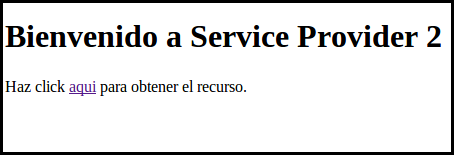
\includegraphics[width=0.6\textwidth]{img/sp2}
\caption{Página inicial del Service Provider 2 sin el cliente autenticado.}
\label{fig:sp2}
\end{figure}
